\section{Interpolation}\label{interpolation}

\subsection{Akima interpolation}\label{akima-interpolation}

Catmull-Rom and Akima interpolation can both be used to get a ``smooth''
transition of a value over the keyframes. These methods can mostly be used
interchangeably, where Akima stays closer to the points where as Catmull-Rom
oscillates a little bit stronger. 5.2 applies to both interpolation forms.

\subsection{Catmul-Rom / Akima interpolation -
	Advices}\label{catmul-rom-akima-interpolation---advices}

\subsubsection{Collision}\label{collision}

Fast approaching the obstacle may cause inadvertent drag to the camera towards
the center of the object. It is recommended to maintain the principle that one
keyframe does not reduce the distance to the object more than 5-times.

\subsubsection{Fly through the gap}\label{fly-through-the-gap}

It is recommended to place a keyframe at the point where the camera flies
through the gap

\subsubsection{Proper conduct cameras between
	objects}\label{proper-conduct-cameras-between-objects}

\subsection{Changing interpolation types}\label{changing-interpolation-types}

To change the interpolation algorithm, right click on the parameter list and the
options appear. In this example the main\_formula\_weight parameters have been
changed from Akima to Linear. Interpolation type is color coded e.g. Linear
parameters are highlighted in grey.

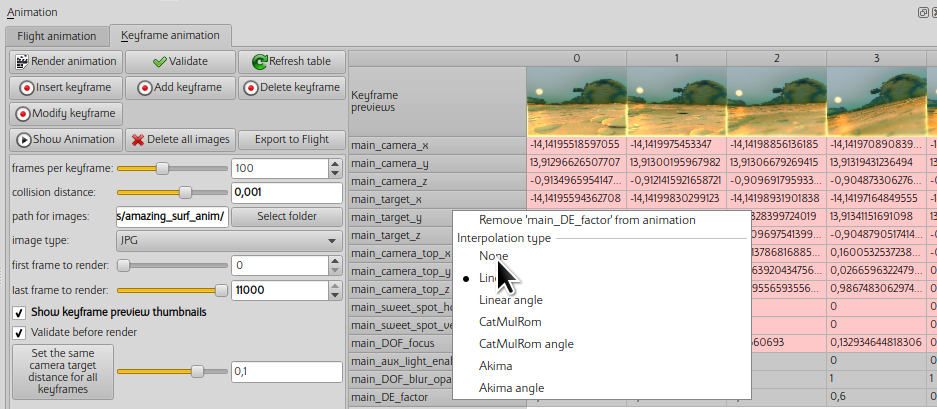
\includegraphics[width=6.69291in,height=2.92087in]{img/manual/media/image26.png}
